\chapter{Technologies and Methods}
\label{sec:tech_and_methods}
This chapter gives a quick introduction to the non-trivial technologies and methods used while developing the system. For purposes of brevity, technologies that are well known or only marginally relevant to the following chapters have been ommited\footnote{Such as CSS3, HTML5, JS ES6, CSS Preprocessors, the vue-router extension, and the Git distributed version control system}. The utilized technologies can roughly be categorized into runtime specific technologies, which are relevant during system execution, and development technologies, which are only relevant while developing, compiling, and testing the system. 
\section{Runtime specific Technologies}
\subsection{Vue.JS ecosystem}
\subsubsection{Vue Framework}
Vue is a Javascript framework used for simplifying the development of reusable, responsive frontend components. The core framework was initially developed by Evan You, in 2014. Since then, the framework quickly gained popularity in the open source community, currently being the 5th most popular open source project on the popular code sharing platform GitHub \cite{GitHubMostStars}. The framework serves a similar purpose as other popular Javascript frontend libraries such as React and Angular, though design, scope, and implementation differences can be found in various places \cite{VueComparisonOtherFrameworks}.
\subsubsection{VueX: State management and Flux Architecture}
The Vue core library is intentionally restricted in scope to the applications view layer. However, a vast Ecosystem has recently emerged around the Vue library covering other required functionalities of modern Web Applications, such as state management, client-side routing, or network connectivity. VueX is a library providing a state management system to the Vue core library which is modelled after Facebooks Flux Architecture \cite{Vuex}\cite{FacebookFlux}. It serves as a centralized store where all application state is located. State can only be retrieved and modified in a predictable fashion. This results in easier maintainability and extensibility for large applications, as developers always know how state is located, accessed, and modified.
\subsubsection{Material Design Components}
Material Design is an open source user interface design system developed and maintained by Google. It consists of design guidelines, components, and development tools. At the time of writing, it is being used in a large quantity of Google products. Furthermore, it is the officially recommended Design Language to use when developing Applications for the Android Platform \cite{AndroidAppQualityGuidelines}. The Design Components are thus familiar and intuitive to use for a large amount of potential end users. The Design Components are available for Vue.JS applications through the vue-material library \cite{VueMaterial}.
\subsection{Reactive Extensions and rx.js}
\gls{RX} is a language agnostic, open source API for asynchronous programming with observable streams. It can be seen as an extension of the Observer pattern \cite{ReactiveXManual}, one of the twenty-three well-known "Gang of Four" design patterns \cite{Gamma:1995:DPE:186897}.

The traditional Observer pattern is based on the fundamental concepts of the \emph{Observable} and the \emph{Observer}. The \emph{Observable} has the ability to \emph{emit} items over time. An \emph{Observer} may declare a dependency on the \emph{Observable} by means of \emph{subscribing} to it. If a subscription has been established, the \emph{Observer} will receive the items as they are emitted from the \emph{Observable}.

The \gls{RX} specification extends on this concept by providing a variety of \emph{Observable operators} to change the emission behavior, transform the emissions, or combine multiple \emph{Observables}.

\begin{figure}[h]
    \centering
    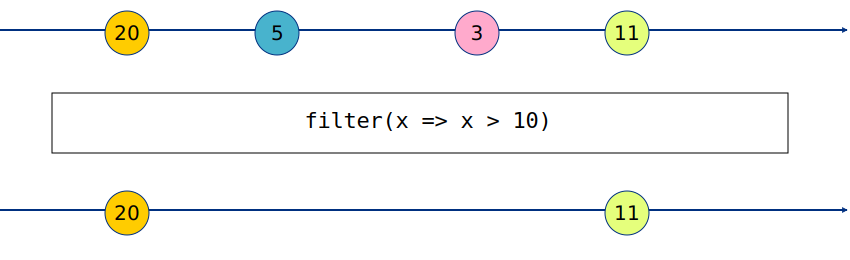
\includegraphics[width=8cm]{filter}
    \caption{An example Observable transformation, represented using \emph{Rx Marble Diagrams}.}
    \label{fig:rx-marbles-filter}
\end{figure}
%
Figure \ref{fig:rx-marbles-filter} gives a visual presentation of an Observable transformation. The top and bottom arrows both represent Observables. The arrow-direction represents time, the colored circles on the arrows represent items emitted by the Observable. The box in the center represents the application of an Observable operator, in this case the \emph{filter} operator, which filters Observable emissions by applying the given predicate, in this example $x > 10$. The result of the transformation is a new Observable that only includes the items that match the given predicate.

Apart from the Observable operators, \gls{RX} also includes specialized versions of the traditional Observable, such as the \emph{Subject}, which has the property of being able to act as Observable and Observer simultaneously, or the \emph{Single}, which represents a singular value emission in the future (similar to the Javascript ES5 Promise).

%
%\subsection{Leap Motion Web Interface
%\subsection{Graphics}
%\subsubsection{THREE.js: Hand Visualization}
%\subsubsection{p5.js: Game Development}
%\subsubsection{d3.js: Dynamic Documents and Visualizations}
%\subsection{Web Specifications}
%\subsubsection{IndexedDB: Persistent Storage}
%\subsubsection{Web Workers: Javascript threading}
%\subsubsection{Service Workers: Offline capability}
%\section{Development specific Technologies}
%\subsection{Webpack: module bundling}
%\subsection{Typescript: static typing}
%\subsection{Inversify: Inversion of Control}
%\subsection{jest and sinon.js: Unit Testing and Mocking}